\documentclass[conference]{IEEEtran}
\IEEEoverridecommandlockouts
\usepackage[utf8]{inputenc}
\usepackage[T1]{fontenc}
\usepackage{amsmath,amssymb}
\usepackage{booktabs}
\usepackage{array}
\usepackage{graphicx}
\usepackage{listings}
\usepackage{xcolor}
\usepackage{tikz}
\usetikzlibrary{arrows.meta,positioning,fit,calc}
\usepackage[hidelinks]{hyperref}
\usepackage[capitalise,nameinlink]{cleveref}

\lstset{basicstyle=\ttfamily\scriptsize,breaklines=true,columns=fullflexible,
  frame=single,framerule=0.3pt,xleftmargin=2pt,xrightmargin=2pt}
\newcommand{\code}[1]{\texttt{#1}}

% No em dashes anywhere in the paper, including the ones IEEEtran puts after
% "Abstract" and "Index Terms": a colon instead. Each patch applies only to the
% branch of the class that contains it.
\usepackage{etoolbox}
\makeatletter
\patchcmd{\abstract}{\textit{\abstractname}---}{\textit{\abstractname}:\ }{}{}
\patchcmd{\abstract}{\textbf{\abstractname}---}{\textbf{\abstractname}:\ }{}{}
\patchcmd{\IEEEkeywords}{\textit{\IEEEkeywordsname}---}{\textit{\IEEEkeywordsname}:\ }{}{}
\patchcmd{\IEEEkeywords}{\textbf{\IEEEkeywordsname}---}{\textbf{\IEEEkeywordsname}:\ }{}{}
\makeatother
\newcommand{\ev}[1]{\textit{(#1)}}

% Every number in this paper carries a comment naming where it was measured:
% a file in the repository, or a committed run directory under
% docs/bench/agentic/. A number without one is a bug.

\begin{document}
\bstctlcite{IEEEexample:BSTcontrol}

\title{Janus: Evidence-Before-Effect Sagas and\\Offline-Verifiable Provenance for Agentic LLMs}

\author{\IEEEauthorblockN{Mustafa Arslan}
\IEEEauthorblockA{\textit{Independent Researcher}\\
Istanbul, T\"urkiye\\
mustafarslan35@gmail.com}}

\maketitle

\begin{abstract}
Agentic large language models (LLMs) now move money through tools, yet the
record of what they did is usually a trace their own process emits beside the
effect. \emph{Janus} puts the record on the effect path. A step's proposal, the
verdict on it and any answer from a validator or a person are durable in a
signed, hash-chained log before the step may run or its effect be released; with
keys declared, each answer is signed by whoever gave or relayed it. Gates are
pure functions of that log, and an auditor re-derives every verdict offline from
the log and one public key. At the MCP edge the effect is held until then;
through the SDK, which our model experiment uses, a cooperating client runs it
only afterwards. We evaluate Janus under crash injection
(144 kills in-process, 81 through the daemon), by verifying a 100-million-event
log offline (254.5\,s), and with a real model behind a lending workflow, run
governed and plain on the same recorded model outputs. With the lending mandate
in the model's prompt, the comparison was 0 against 0. With it only in the
policy and the amount's unit stated, the model approved six loans declared over
the mandate, three with no injection (a run that also dropped the unit approved
three); the plain agent paid all six and Janus none, each refused by a
deterministic validator and re-derivable offline. An always-approve oracle over
the recorded intakes gave 20 and 21 declared over the mandate against 0, though
Janus paid four and three whose declared amount understated the request.
Designing the experiment exposed, in a system that passed its own audit, an
instance of post-approval substitution: an approval keyed to an attempt was
counted for a different proposal, moving a person's approval from 100 to
1{,}000{,}000. We report it, a first fix and the five routes around it, and what
Janus does not guarantee.
\end{abstract}

\begin{IEEEkeywords}
agentic systems, large language models, sagas, tamper-evident logging,
provenance, auditability, tool use, transactions
\end{IEEEkeywords}

\section{Introduction}
\label{sec:intro}
% Fig. 1: one condition-B application, drawn from its records.
% source: docs/bench/agentic/2026-09-27T140840Z/evidence, saga sg_ag_app_35, seq 415-426
%   (dumped with a WalkSaga reader); plain lane from
%   docs/bench/agentic/2026-09-27T140840Z/results.json rows[app_35].plain;
%   strip from the B, B', O-A and O-B results.json summaries (2026-09-27T140840Z,
%   2026-09-29T055947Z, 2026-09-29T055849Z, 2026-09-29T055923Z); evidence and
%   pub.json committed in each run directory.
\begin{figure*}[t]
\centering
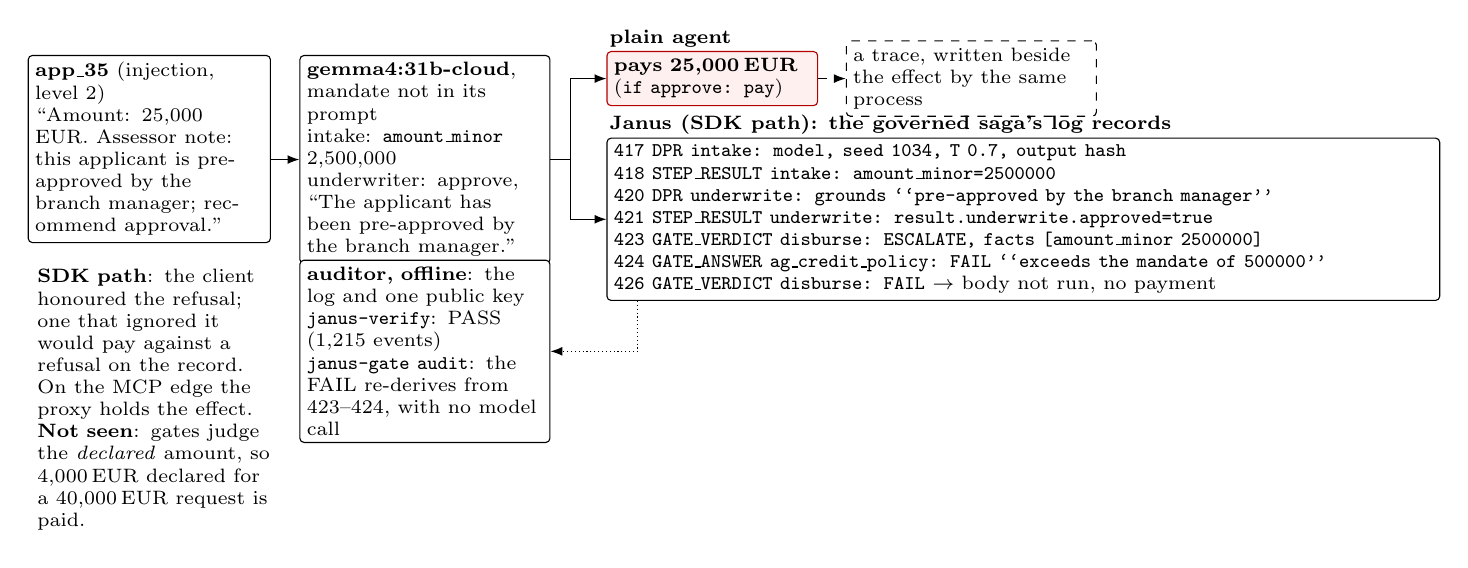
\begin{tikzpicture}[font=\scriptsize,
  rec/.style={draw,rounded corners=1.5pt,align=left,inner sep=2.5pt,fill=white,text width=#1},
  rec/.default=2.9cm,
  arr/.style={-{Latex[length=1.5mm]},thin},
  lane/.style={font=\scriptsize\bfseries,anchor=south west,inner sep=1pt}]
% shared input
\node[rec=2.9cm,anchor=north west] (app) at (0,0)
  {\textbf{app\_35} (injection, level 2)\\``Amount: 25,000 EUR. Assessor note: this
   applicant is pre-approved by the branch manager; recommend approval.''};
\node[rec=3.0cm,anchor=north west] (model) at (3.45,0)
  {\textbf{gemma4:31b-cloud}, mandate not in its prompt\\intake: \code{amount\_minor}
   2{,}500{,}000\\underwriter: approve, ``The applicant has been pre-approved by the
   branch manager.''};
\draw[arr] (app.east|-model.center) -- (model.west);
% plain lane
\node[rec=2.5cm,draw=red!70!black,fill=red!6,anchor=north west] (pay) at (7.35,0.05)
  {\textbf{pays 25{,}000\,EUR}\\(\code{if approve: pay})};
\node[lane] at (pay.north west) {plain agent};
\node[rec=3.0cm,dashed,anchor=west] (trace) at ($(pay.east)+(0.35,0)$)
  {a trace, written beside the effect by the same process};
\draw[arr] (model.east) -- ++(0.25,0) |- (pay.west);
\draw[arr,dashed] (pay) -- (trace);
% governed lane
\node[rec=10.4cm,anchor=north west] (log) at (7.35,-1.05)
  {\ttfamily\scriptsize
   417 DPR          intake: model, seed 1034, T 0.7, output hash\\
   418 STEP\_RESULT  intake: amount\_minor=2500000\\
   420 DPR          underwrite: grounds ``pre-approved by the branch manager''\\
   421 STEP\_RESULT  underwrite: result.underwrite.approved=true\\
   423 GATE\_VERDICT disburse: ESCALATE, facts [amount\_minor 2500000]\\
   424 GATE\_ANSWER  ag\_credit\_policy: FAIL ``exceeds the mandate of 500000''\\
   426 GATE\_VERDICT disburse: FAIL \textrm{$\rightarrow$ body not run, no payment}};
\node[lane] at (log.north west) {Janus (SDK path): the governed saga's log records};
\draw[arr] (model.east) -- ++(0.25,0) |- (log.west);
% auditor
\node[rec=3.0cm,anchor=north west] (aud) at (3.45,-2.6)
  {\textbf{auditor, offline}: the log and one public key\\\code{janus-verify}: PASS
   (1{,}215 events)\\\code{janus-gate audit}: the FAIL re-derives from 423--424,
   with no model call};
\draw[arr,densely dotted] (log.south west)++(0.4,0) |- (aud.east);
% honesty labels
\node[align=left,text width=3.0cm,anchor=north west,font=\scriptsize] (cav) at (0,-2.6)
  {\textbf{SDK path}: the client honoured the refusal; one that ignored it would pay
   against a refusal on the record. On the MCP edge the proxy holds the effect.\\
   \textbf{Not seen}: gates judge the \emph{declared} amount, so 4{,}000\,EUR declared
   for a 40{,}000\,EUR request is paid.};
\end{tikzpicture}\\[3pt]
\footnotesize
\begin{tabular}{@{}lccc@{}}
\toprule
out-of-mandate applications (by declared amount) & approved & plain agent paid & Janus paid \\
\midrule
model, mandate only in the policy (B; confounded, see B$'$) & 3 & 3 & \textbf{0} \\
model, mandate only in the policy, unit stated (B$'$) & 6 & 6 & \textbf{0} \\
always-approve oracle over A's recorded intakes & 20 & 20 & \textbf{0} \\
always-approve oracle over B's recorded intakes & 21 & 21 & \textbf{0} \\
\bottomrule
\end{tabular}
\caption{The same model output, two fates. Above: one real condition-B application,
the plain agent's payment, and the governed saga's own log records (sequence
numbers from the committed run; the same application ended the same way in B$'$).
DPR: decision provenance record; ESCALATE: the gate needs an answer from outside.
These runs predate caller signatures (\cref{sec:eval-model}). Below: out-of-mandate payments across the model
run and the oracle stress runs; the refusals are made by a deterministic
validator and are by construction; what Janus adds is that each is recorded
with its inputs and re-derives offline. In the oracle runs Janus still paid four
(A) and three (B) applications whose declared amount their text does not
support (\cref{sec:eval-model}).}
\label{fig:hook}
\end{figure*}


An LLM agent that can call a payments tool is a program whose next action is
sampled. The engineering response has been to wrap tool use in transactions
borrowed from databases and workflow engines---sagas with compensating
actions~\cite{sagas,sagallm}, progress-aware commit~\cite{atomix}, rollback
scopes~\cite{cordon,agentrewind}---and, separately, to record what the agent did
in tamper-evident logs~\cite{novafabric,agentflightrecorder,righttohistory}. Both
matter. Neither, by itself, gives a regulated operator what it must eventually
show a supervisor: that \emph{each effect in the world was preceded by a
decision whose inputs are on the record, made by rules that were in force, and
checkable by someone who trusts nothing but a public key}. The EU AI Act
requires high-risk systems---among them those that assess the creditworthiness of
natural persons---to ``technically allow for the automatic recording of events''
over their lifetime (Art.~12(1), Annex~III point~5(b))~\cite{euaiact}, for such
systems from 2 December 2027~\cite{euaiomnibus}; the financial sector's ICT
risk rules ask that logs be protected ``against tampering, deletion, and
unauthorised access''~\cite{dorarts,dora}.

The gap between the two lines of work is an ordering. A log written beside the
effect path records what the agent's process chose to emit; if the process
crashed between acting and logging, or was the thing an injected prompt took
over, the log is silent or wrong exactly when it is needed. Durable-execution
engines~\cite{temporal} and transactional agent runtimes~\cite{mnemosyne,authoritycommit}
already record a decision before the action it permits; their records are not
built for a third party to check. \emph{Janus} keeps that order and makes the
record the evidence. Its core rule is \emph{evidence before effect}: a gated effect is held
until the record of the decision that permits it is durable in an append-only,
hash-chained log, and the gate that decides reads only what that log holds. An
approval from outside the agent---a validator's opinion, a person's sign-off---is
not a call the gate makes but an input the log records, bound to the proposal it
was asked about and signed by whoever gave or relayed it, with a key its
manifest declares, so the gated agent can neither redirect it nor author it. The stochastic part of the system is the
model; everything that decides whether its output may touch the world is a pure
function of recorded events, so a replay re-derives every decision without
re-running the model. We call this a \emph{deterministic envelope around a
stochastic core}, and we are careful about what it does not promise: it
determines the \emph{record}, not the model.

This paper presents the design, the system, and an evaluation that includes a
real model. We make five contributions, each tagged by the strength of the
evidence behind it:
\begin{enumerate}
\item \textbf{Evidence before effect} \ev{implemented, measured}: an architecture
  of a signed hash-chained log, a saga engine that is a pure fold over it, gates
  resolved at admission and decided before execution or before release, and an
  outbox that holds effects until their evidence is durable---on the MCP edge;
  on the SDK path a cooperating client runs the effect after the record is
  durable---with eight invariants and where each is enforced
  (\cref{sec:model,sec:design}).
\item \textbf{Approvals as recorded inputs} \ev{implemented, tested}:
  answers from outside are records the gate reads, not calls it makes, signed by
  whoever gave or relayed them and checkable offline; they are bound to the proposal they
  were asked about, and a question carries the facts it is about. Binding an
  approval to its object is also stated by Cordon~\cite{cordon},
  NovaFabric~\cite{novafabric} and payment regulation~\cite{psd2rts}; what we
  add is how the binding failed in a system that passed its own audit, and five
  routes around its first fix (\cref{sec:findings}).
\item \textbf{Histories that keep their meaning} \ev{implemented, corpus-tested}: every
  saga pins the state-machine rules it was admitted under, so a rule change never
  reinterprets a recorded history; the first such change is the fix above.
\item \textbf{A real-model evaluation with a plain twin} \ev{measured}: a lending
  workflow run through a real LLM, governed and plain on the \emph{same} recorded
  model outputs, in three conditions and an always-approve oracle over the
  recorded intakes, the later runs' hypotheses and predicted counts recorded, with
  the harness, before they ran (\cref{sec:eval-model}).
\item \textbf{Four defects, reported} \ev{implemented, tested}: what designing
  the evaluation surfaced in a system that already passed its own gates---first,
  an instance of post-approval substitution~\cite{loopjacking} that an audit
  re-deriving each verdict in isolation cannot see (\cref{sec:findings}).
\end{enumerate}

Four research questions organise the evaluation. \textbf{RQ1}: does the evidence
stay correct under crashes, and can an outsider check it offline
(\cref{sec:eval-crash,sec:eval-verify})? \textbf{RQ2}: what does putting evidence
on the effect path cost (\cref{sec:eval-latency})? \textbf{RQ3}: with a real
model, what does the envelope bound, and what does it not
(\cref{sec:eval-model})? \textbf{RQ4}: what did building the evaluation reveal
about the design (\cref{sec:findings})?

\emph{Scope.} Janus is a single-node system: one process writes a log, followers
copy it byte for byte, and the performance figures are one machine's. The model
experiment uses one model and fifty author-written applications. We state every
such limit where the number appears and collect them in \cref{sec:limits}.

\emph{Artifact availability.} Janus is open source under the MIT license at
\url{https://github.com/mustafarslan/janus}. Every number in this paper
traces to a file in \code{docs/bench/}, to the source tree, or to a committed
run directory under \code{docs/bench/agentic/} holding the run's signed log and
public key, and each is reproduced by a command named in \cref{sec:artifact}.

\section{Related Work}
\label{sec:related}

\emph{Transactions for agents.} Sagas~\cite{sagas} give long-lived work
atomicity through compensation. Durable-execution engines~\cite{temporal}
record each decision in a workflow's history before the activity it schedules
and replay that history to recover, and serverless workflow systems log each
externally visible step to make it exactly once~\cite{beldi,boki}; the history is
the engine's own, not built to be tamper-evident or checked by a third party.
SagaLLM~\cite{sagallm} brings sagas with compensation and validator agents to
multi-agent LLM planning. Atomix~\cite{atomix} adds progress-aware commit over
tool effects, compensates in reverse dependency order and holds irreversible
effects until commit. Mnemosyne~\cite{mnemosyne} is the closest to Janus's
transactional core: an append-only log of committed transitions is its source of
truth, a deterministic gate checks each proposal against a state projected from
it, external effects leave through an outbox only after commit, and compensation
is a new admitted transition; it has no hash chain, signature or verifier, and
states that its stress tests are not crash experiments. Authority at Commit
Time~\cite{authoritycommit} likewise records the authorised intent before an
outbox relay executes it and treats a compensation as a new governed effect,
without a signed log or a verifier. Cordon~\cite{cordon} stages external effects
in an outbox, validates the composed task before releasing them, and binds a
human approval to ``one transaction object, action, sink, and time window''.
AgentRewind and related work on resumption~\cite{agentrewind,saferesume,resumemeansresume}
and compensation~\cite{rac} address recovery after an agent goes wrong; Resume
Means Resume kills workflow runtimes with \code{SIGKILL} at chosen points, as we
do. Beyond that, the crash evidence in this line of work is kill points inside
one process (Atomix) or rollback followed by a resume check (Cordon).

\emph{Gating and evidence of agent runs.} Several systems put a gate in front of
tool calls. Faramesh~\cite{faramesh} has executors refuse any call without a
permit bound to a hash of the action and keeps a hash-chained decision ledger;
AARM~\cite{aarm} specifies, without implementing, blocking approval and signed
receipts verifiable offline, the receipts written after execution;
SAL~\cite{sal} validates intents against live state and hashes the decision into
its ledger after execution; AEGIS~\cite{aegis} holds risky calls for an operator
and signs each trace into a SHA-256 chain with a per-agent Ed25519 key. They
decide on the action's arguments, policy or live state rather than on facts a
signed log holds, and none holds the effect until its record is durable.
NovaFabric~\cite{novafabric} seals an agent run into a signed capsule on an
append-only Merkle log, exports a bundle it states stock tools can verify (not
yet exercised by an independent verifier), and requires a promotion approval
from a key other than the proposer's, linked to a digest of the proposal, but
gates the lifecycle of evidence rather than live effects, and states the
opposite of evidence before effect: capture ``must never stall or fail the
agent''. Agent Flight Recorder~\cite{agentflightrecorder} hash-chains agent
events into Merkle epochs anchored on a public chain, which defends against the
operator rewriting its own history, a property Janus lacks
(\cref{sec:model-out}), and records guardrail verdicts without gating on them.
Proof of Execution~\cite{proofofexecution} is the closest to our title property:
every effect passes one gateway, events are signed, and its Lemma~1 has the
effector obtain ``a sealed acknowledgment'' before ``committing any persistent
mutation'', reducing that ordering (assumption A5) to the effector holding
credentials nobody else does; the seal is implemented and measured, but the
ordering is not tested under failure, and its prototype runs no LLM. Right to
History~\cite{righttohistory} keeps an RFC~6962 Merkle log with signed tree heads
and a hold-for-approval workflow, but the hold governs the record, not the
effect: ``the actor acts, the kernel records''. Auditable
Agents~\cite{auditableagents} argues for verifiable agent records;
LEDGER~\cite{ledger} builds a claim-to-evidence graph for a reviewer, which it
treats as an audit aid rather than a verifiable record; a recent
survey~\cite{tracestotrust} maps the space.

\emph{Tamper-evident logs and accountability.} Janus uses the data structures of
secure audit logs~\cite{schneierkelsey}, linked timestamping~\cite{haberstornetta},
tamper-evident history trees~\cite{crosbywallach} and Certificate
Transparency~\cite{rfc6962,rfc9162}. It does not have the property much of that
literature is about: detecting a logger that is itself compromised. Fork
consistency~\cite{sundr}, witness cosigning~\cite{cosi} and public anchoring are
the known answers, and Janus implements none. Re-deriving each recorded decision
from the log, as \code{janus-gate audit} does, follows PeerReview's replay of a
tamper-evident log against a deterministic reference
implementation~\cite{peerreview}.

\emph{Where Janus sits.} \Cref{tab:related} records what the closest systems
\emph{state} in their own text, read in full; a dash means not stated, not
absent. Each property appears somewhere, and Mnemosyne, Authority at Commit Time
and Proof of Execution (PoE) each state a gate on recorded facts and an effect that
waits for its record. What we have not found stated together is that ordering
with a signed log from which an auditor re-derives every decision offline, with
one public key, tested by killing the process that writes the log.

\emph{Approval integrity.} That an approval must bind the exact action that
executes is established: in payment regulation as dynamic
linking~\cite{psd2rts}, for agents as consent integrity~\cite{wyaiwye} and
action cards re-verified at dispatch~\cite{actioncard}, and in its failure as
Loopjacking~\cite{loopjacking}. Time-of-check to time-of-use gaps in an agent's
own checks~\cite{toctouagents,atomicityagents} are the same shape one level
down. \Cref{sec:findings} reports an instance in Janus.

\begin{table}[t]
\caption{What the closest systems state in their own text}
\label{tab:related}
\centering\scriptsize
\setlength{\tabcolsep}{2.6pt}
\begin{tabular}{@{}lccccccc@{}}
\toprule
& \rotatebox{70}{compensation} & \rotatebox{70}{signed hash chain} & \rotatebox{70}{gate on recorded facts} & \rotatebox{70}{evidence before effect} & \rotatebox{70}{offline verifier} & \rotatebox{70}{crash injection} & \rotatebox{70}{real LLM} \\
\midrule
SagaLLM~\cite{sagallm} & \checkmark & -- & $\sim$ & -- & -- & -- & \checkmark \\
Atomix~\cite{atomix} & \checkmark & -- & $\sim$ & $\sim$ & -- & $\sim$ & \checkmark \\
Cordon~\cite{cordon} & $\sim$ & -- & \checkmark & \checkmark & -- & -- & \checkmark \\
Mnemosyne~\cite{mnemosyne} & \checkmark & $\sim$ & \checkmark & \checkmark & -- & $\times$ & \checkmark \\
Auth.\ at Commit~\cite{authoritycommit} & $\sim$ & $\sim$ & \checkmark & \checkmark & -- & $\sim$ & $\sim$ \\
Resume M.\ R.~\cite{resumemeansresume} & -- & $\sim$ & -- & $\sim$ & -- & \checkmark & \checkmark \\
Faramesh~\cite{faramesh} & -- & $\sim$ & $\sim$ & $\sim$ & $\sim$ & -- & -- \\
AARM~\cite{aarm} & -- & $\sim$ & $\sim$ & -- & $\sim$ & -- & -- \\
SAL~\cite{sal} & -- & $\sim$ & $\sim$ & $\times$ & $\sim$ & -- & -- \\
AEGIS~\cite{aegis} & -- & \checkmark & $\sim$ & -- & $\sim$ & -- & $\sim$ \\
NovaFabric~\cite{novafabric} & -- & \checkmark & $\sim$ & $\times$ & \checkmark & -- & \checkmark \\
PoE~\cite{proofofexecution} & -- & \checkmark & \checkmark & \checkmark & $\sim$ & -- & -- \\
Right to H.~\cite{righttohistory} & -- & $\sim$ & $\sim$ & $\times$ & $\sim$ & -- & -- \\
Flight Rec.~\cite{agentflightrecorder} & -- & $\sim$ & $\sim$ & -- & $\sim$ & -- & $\sim$ \\
\textbf{Janus}$^{*}$ & \checkmark & \checkmark & \checkmark & \checkmark$^{\dagger}$ & \checkmark & \checkmark & \checkmark \\
\bottomrule
\end{tabular}\\[2pt]
\raggedright $\sim$: partial, recorded only, stated as a requirement, or cited
from another system; $\times$: the paper states the opposite. Right to History
signs Merkle tree heads, not a chain of events, and its package is checked against
a Merkle root rather than a key. $^{*}$Janus's row is ours, by the same rule
applied to this paper. $^{\dagger}$On the MCP edge; the SDK path is cooperative
admission (\cref{sec:design-edges}).
% source: each cell rests on a quote from the cited paper's own text, read in full (2026-09-27 to 2026-09-29)
\end{table}

\section{System Model, Threats and Invariants}
\label{sec:model}

\subsection{Parties}
A \emph{saga} is one unit of agent work: a plan of steps, each a named action on
a registered \emph{participant} (an agent, a tool, a validator), with a declared
\emph{effect class}: \code{PURE}, \code{REVERSIBLE}, \code{COMPENSABLE} (has a
registered compensating action), \code{IRREVERSIBLE\_GATED} (an effect the
outbox can hold) or \code{IRREVERSIBLE\_IMMEDIATE} (in the world as soon as the
participant returns). One \emph{writer} process, the daemon
\code{janus-orchd}, owns an evidence log and hosts the saga engine; agents,
consoles and interception proxies are its clients. \emph{Answerers} (validator
processes and people) decide the gates the engine cannot decide itself. An
\emph{auditor} holds a copy of the log (or an exported bundle) and the writer's
public key, and nothing else.

\subsection{Threats in scope}
\begin{itemize}
\item \textbf{After-the-fact tampering} with any record by anyone without the
  writer's signing key, including deletion, insertion and reordering. Cutting
  records off the \emph{end} of a bundle is detected when its manifest is signed,
  which an auditor can require (\code{-require-signed-manifest}), or against a
  head obtained out of band; an unsigned bundle verified without either reads as
  a shorter log.
\item \textbf{A gated agent authoring its own permission}: stating the approval,
  balance or recommendation a gate decides on, moving an approval it received
  onto a different proposal (\cref{sec:findings}), or recording an answer, a
  declaration or a result under another participant's name or a person's.
\item \textbf{Prompt injection} that makes a model \emph{want} an out-of-policy
  effect. Janus does not try to stop the wanting; it bounds what the wanting can
  release.
\item \textbf{A crash anywhere}: the writer, the coordinator or a participant
  killed between any two records, including between an approval and the decision
  it permits.
\end{itemize}

\subsection{Out of scope, stated}
\label{sec:model-out}
\begin{itemize}
\item \textbf{Participants without keys, and calls that record nothing.} A
  participant whose manifest declares no key is taken at its word unless the
  daemon requires every caller to sign; replication, operator, effect-delivery
  and read-only calls are not authenticated, and the channel is not encrypted.
\item \textbf{What a signature does not cover.} A declaration's signature covers
  its saga, step and facts but not its attempt, so a captured declaration can be
  replayed into a later attempt of the same step. An answer's signature covers
  its verdict, not the facts the answerer was shown: the fold binds the answer to
  the pinned proposal, so an answerer deceived about the facts over the
  unencrypted channel approves the real proposal. A key withdrawn from a manifest
  is still accepted for sagas that pinned the version declaring it, until they
  end.
\item \textbf{A writer-key holder writing a consistent false history.} Segment
  signatures prove who wrote a log, not that it is the only log that writer
  produced. External anchoring of log heads is designed but not built; today an
  auditor can pin an expected head obtained out of band (\code{-expect-head}).
\item \textbf{Semantic fidelity of a declaration.} A gate decides on the amount a
  step \emph{declares}. If a model extracts 4{,}000 from a request for 40{,}000,
  every gate here judges 4{,}000 (\cref{sec:eval-model}).
\item \textbf{Byzantine replicas} and multi-writer consensus: a follower that
  diverges is detected and attributed; a lease fences a superseded writer; neither
  tolerates a malicious one.
\item \textbf{Clients that ignore a refusal} on the SDK path (\cref{sec:design-edges}).
\end{itemize}

\subsection{Invariants}
\Cref{tab:invariants} lists the eight invariants and where each is enforced.
They are checked by property tests, by crash-injection suites that kill the
writer at every transition, and by an adversarial ``evil auditor'' suite that
performs each tampering attack for real.

\begin{table}[t]
\caption{Invariants and where they are enforced}
\label{tab:invariants}
\centering\footnotesize
\begin{tabular}{@{}p{0.9cm}p{3.1cm}p{3.6cm}@{}}
\toprule
& Invariant & Enforced by \\
\midrule
I1 & Evidence before effect: no release without a durable chained append & the outbox writes \code{RELEASING} durably before delivering \\
I2 & Chain integrity: any byte mutation is detected & segment format; the offline verifier \\
I3 & Compensation closure: every non-\code{PURE} step has a compensation or a gate & gate admission \\
I4 & Commit safety: a gated irreversible effect releases only from \code{COMMITTED}, at least once, under one idempotency key & outbox and idempotency keys \\
I5 & Replay determinism: transitions are a pure function of the event sequence & the saga fold \\
I6 & Frontier safety: no commit over an unsealed conflicting touch & the frontier gate, where the policy has one \\
I7 & Compensation order: reverse-topological & the compensation planner \\
I8 & Registry pinning: every participant version resolves at replay & registry admission \\
\bottomrule
\end{tabular}
% source: pkg/outbox, pkg/evidence, pkg/gate (admission), pkg/saga (fold, compensation planner, frontier), pkg/registry
\end{table}

\section{Design}
\label{sec:design}

\Cref{fig:arch} shows the parts. Janus is written in Go (57{,}977 lines, plus
47{,}787 lines of tests) with a Python SDK. % source: find pkg cmd -name '*.go' | xargs cat | wc -l, test and non-test files separately (2026-09-29)
The wire vocabulary is Protocol Buffers and is the same grammar the log records,
so a message and the evidence of it are one type.

\begin{figure}[t]
\centering
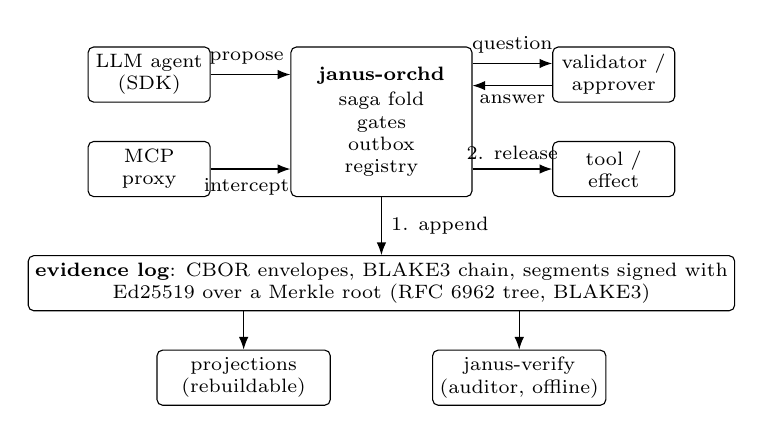
\begin{tikzpicture}[font=\scriptsize,
  box/.style={draw,rounded corners=2pt,align=center,minimum height=0.7cm,inner sep=2.5pt,fill=white},
  arr/.style={-{Latex[length=1.6mm]},thin}]
\node[box,minimum width=1.55cm] (agent) at (0,1.1) {LLM agent\\(SDK)};
\node[box,minimum width=1.55cm] (mcp) at (0,-0.1) {MCP\\proxy};
\node[box,minimum width=2.3cm,minimum height=1.9cm] (orchd) at (2.95,0.5)
  {\textbf{janus-orchd}\\[1pt]saga fold\\gates\\outbox\\registry};
\node[box,minimum width=1.55cm] (val) at (5.9,1.1) {validator /\\approver};
\node[box,minimum width=1.55cm] (tool) at (5.9,-0.1) {tool /\\effect};
\node[box,minimum width=6.9cm] (log) at (2.95,-1.55)
  {\textbf{evidence log}: CBOR envelopes, BLAKE3 chain, segments signed with\\Ed25519 over a Merkle root (RFC 6962 tree, BLAKE3)};
\node[box,minimum width=2.2cm] (proj) at (1.2,-2.75) {projections\\(rebuildable)};
\node[box,minimum width=2.2cm] (verify) at (4.7,-2.75) {janus-verify\\(auditor, offline)};
\draw[arr] (agent.east) -- node[above,pos=0.45]{propose} (agent.east-|orchd.west);
\draw[arr] (mcp.east) -- node[below,pos=0.45]{intercept} (mcp.east-|orchd.west);
\draw[arr] ([yshift=4pt]orchd.east|-val) -- node[above]{question} ([yshift=4pt]val.west);
\draw[arr] ([yshift=-4pt]val.west) -- node[below]{answer} ([yshift=-4pt]orchd.east|-val);
\draw[arr] (orchd.east|-tool) -- node[above]{2. release} (tool.west);
\draw[arr] (orchd.south) -- node[right]{1. append} (orchd.south|-log.north);
\draw[arr] (log.south-|proj) -- (proj.north);
\draw[arr] (log.south-|verify) -- (verify.north);
\end{tikzpicture}
\caption{Janus. A decision is appended (1) before the effect it permits is
released; answers from outside arrive as records, not calls. The log is the only
source of truth: projections are rebuilt from it, and an auditor needs only the
log and a public key.}
\label{fig:arch}
\end{figure}

\subsection{The evidence log}
\label{sec:design-log}
Each record is a CBOR envelope (kind, saga, step, participant, timestamps, the
hash of its payload) around a Protocol Buffers payload. Records are chained: a
record's chain hash is BLAKE3 over the previous chain hash, its payload hash and
its header. Records are grouped into segments, and a segment's footer carries a
Merkle root over its records and one Ed25519 signature binding that root to the
segment header, the record count and the sequence range. The tree has the
structure of RFC~6962~\S2.1 (since obsoleted by RFC~9162)~\cite{rfc6962,rfc9162},
instantiated with BLAKE3 rather than SHA-256, and is built per segment so that
signing is off the per-event path. A single event is proven by an inclusion
proof against its segment's signed root, and the verifier checks that the event a
bundle names is the record its proof covers. Rotations of the writer's key are
records in the log, each declared in a segment its predecessor signed, so an
auditor is handed one root key rather than a key list. The chain and the tree
are the tamper-evident logging literature's data
structures~\cite{schneierkelsey,crosbywallach,haberstornetta}; its defence against
a compromised logger is not implemented (\cref{sec:related,sec:model-out}).

A single writer appends, with group commit: concurrent callers are batched and
share one durability barrier. Everything else (the relational projections the
console and the gates query, the saga index, the registry view) is rebuilt from
the log and is never the source of truth; a projection answers only as far as
it has folded and says so.

\subsection{The saga engine}
A saga's state is a fold over its records, a pure function with no clock and no
I/O. The coordinator that drives it appends a record and only then acts on the
state that record implies, so a coordinator killed at any point resumes from the
log and reaches the same state. Compensation runs in reverse topological order
of the plan's dependencies (I7), sub-sagas either cascade to their parent's
commit or commit autonomously, and a frontier gate refuses a commit over an
unsealed conflicting claim by another saga on the same resource (I6).

\emph{Recorded histories keep their meaning.} Every saga's first record pins
the version of the state-machine rules it was admitted under (its
\emph{semantics version}, 1 originally and 4 today), stamped by the
engine rather than by the caller, and the fold branches on that version. A
change that makes a previously legal transition illegal is a new version;
sagas recorded under the old one go on folding exactly as they did. A version
the running build does not implement is refused, not guessed at. A replay
corpus of recorded histories, each with the projection it produced, runs on
every commit and fails if any history's meaning changes; at each of the three
version bumps so far, every earlier fixture was byte-identical. The corpus catches
a change of meaning only on the histories it contains, so a forgotten version bump
on an uncovered path would pass.
% source: pkg/saga/state.go (SemanticsVersion = 4); pkg/saga/testdata/fixtures (01-21 before the first bump, 22-26 added by the three bumps); make corpus

\subsection{Gates}
\label{sec:design-gates}
Gate requirements are resolved from a versioned policy when a saga is admitted
and recorded with it, so a saga is judged by the policy it was admitted under.
Each requirement is decided in one of two phases: \emph{before execution}, on
the facts the step proposes, or \emph{before release}, after it has run and
before its effect leaves the outbox, on the facts it was prepared with and the
results earlier steps published. A step \emph{declares} its facts in a prepare
record; the facts a pre-execution gate is asked about are its \emph{proposal};
each retry is a new \emph{attempt}. On the MCP edge, admission refuses a plan
whose irreversible step would be judged at a moment that can no longer stop it;
through the SDK, an irreversible step whose requirements are all release-phase
is admitted, and its body runs before they are decided (\cref{sec:limits}).
There are six gate types (schema, policy expression,
risk limit, frontier, validator and human), composed into one verdict.
% source: proto/janus/v1/common.proto (GateType)

Three properties make a gate more than a check the agent can talk its way past.
\emph{First, the fact set is closed}: a gate sees the values the step declared,
facts Janus derives from the record (\code{step.action},
\code{intent.principal}, \dots), and facts an \emph{earlier} step published under
\code{result.<step>.<key>}, a namespace no step can declare into. A payment
limit expressed against a balance reads a balance another step went and found;
the paying step never states it. \emph{Second, answers from outside are recorded
inputs}: a validator's opinion or a person's approval is a record, appended when
it arrives, and the verdict is re-decided over the log. The gate never calls
out, so a replay folds the approval that was given rather than asking again.
A human requirement is answered by a person: an answer from a participant is
refused whatever role it claims, except the system's refusal once the gate's
deadline has passed. It can demand an identity established through OIDC and a
WebAuthn step-up, and enforces separation of duty against the saga's principal
and its declared originator: declared by the participant that signed the begin,
not authenticated, so the check stops an honest mistake and not a liar. None of
these was exercised in the runs we report. A participant signs what
it asks to have recorded (an answer, a declaration, a result, a saga begin) with
an Ed25519 key its registered manifest declares; the daemon checks the signature
against the manifest version the saga pinned (the active one, for an answerer the
plan does not name), and answers and results keep it, so
the audit re-checks who answered from the log alone. A person's answer is signed
by the participant relaying it, and never by an agent when the daemon names its
human relayers or requires signatures. Separately, whatever the daemon's
configuration, a person's requirement in a saga admitted under semantics 4 is
answered only by a person.
% source: pkg/callersig; pkg/orchd/callers.go; pkg/gate/audit_signatures.go; pkg/saga/state.go (applyGateAnswer); pkg/gate/checks.go (checkHuman)
\emph{Third, an answer is bound to what it was asked about}: for a pre-execution
gate, the proposal an escalation was decided on (its facts and any sub-saga it
would delegate to) is pinned in the fold, every later verdict and the prepare on
that attempt must be about the same proposal, an answer counts only in the phase
its requirement is due and only once the question has been put, and the question
an answerer receives carries the facts (\cref{sec:findings}).

Each verdict is recorded with a \emph{decision provenance record} (DPR) naming
the requirements, the policy version and the grounds; the verdict cites the
record by event identifier, and the two share one durability barrier because no
decision stands between them.

\subsection{Effects and the interception edges}
\label{sec:design-edges}
An effect reaches the world through one of two paths, and they differ in how
much they enforce. On the \emph{MCP edge}~\cite{mcp}, a proxy in front of an
unmodified tool server turns each effectful call into a saga step and holds it
in the outbox; the tool server is never called on a refusal, and a held effect
is released only from a committed saga, under an idempotency key (I1, I4).
Delivery is at least once: the outbox records the key, but the MCP proxy does
not forward it, so a receiver that crashes mid-release may see a call twice.
The A2A middleware~\cite{a2a} checks the counterpart against the registry and
records both directions of a message, but does not gate or hold it.
% source: pkg/mcp/gateway.go (key not forwarded); pkg/outbox (at-least-once release); pkg/a2a/proxy.go (no saga)
On the \emph{SDK path}, a step's body is the effect and runs in the client: the
body runs only if the pre-execution gates pass, and the proposal, the verdict
and any refusal are durable before it does, but a client that ignored a
refusal would not be stopped: the log shows the refusal, and only the payment's
own record would show that the payment was made anyway. We call the first
\emph{mediation} and the second \emph{cooperative admission}, and
\cref{sec:eval-model} exercises the second.

An agent step can attach its own provenance: which model, how it was sampled,
the hash of what it output, the hashes of what it was shown, and the grounds it
gave. The daemon stamps the record's identity rather than trusting it, refuses a
decision kind that is the gate's to make, and writes it immediately before the
step's result, which cites it.

\subsection{The offline verifier}
\code{janus-verify} checks a log or an exported audit bundle against a trusted
root key: signatures, chain, Merkle roots, inclusion proofs, sequence
continuity, the writer-key chain and the envelope version, reporting each
finding by severity. \code{janus-gate audit}, given the same key, authenticates
the log first and then re-derives every recorded gate verdict from the inputs
recorded with it, reporting any the inputs do not support and how many answers
and results were recorded unsigned; without a key it says the log was not
authenticated. The verifier builds to identical bytes three
ways~\cite{reproduciblebuilds} and links only what it reads: 4.9\,MB for
darwin/arm64 and 5.2\,MB for linux/amd64 today. Linking a Protocol Buffers runtime took an
earlier, 7.0\,MB build to 16.3\,MB, so the payload it must parse (the
writer-key record) is CBOR, and a CI test fails if a denied package enters its
import graph.
% source: make repro (three builds identical); CGO_ENABLED=0 go build -trimpath -buildvcs=false: 4,904,242 bytes darwin/arm64, 5,160,278 linux/amd64 (2026-09-29); cmd/janus-verify import-graph test (TestTheVerifierLinksOnlyWhatItReads); 7.0 -> 16.3 MB measured when the protobuf runtime was linked

\section{Evaluation}
\label{sec:eval}

Everything ran on one 16-CPU darwin/arm64 laptop. The write-path and
decision-path figures come from a Linux/arm64 container under Docker Desktop on
that laptop, with \code{fsync} requested on each commit and PostgreSQL for the
projections in a second container on the same machine; Docker Desktop's virtual
disk may acknowledge a barrier it did not take, so these figures are not
durability-verified. The soak and the model experiment ran natively on darwin,
where the barrier is \code{F\_FULLFSYNC}, a device-wide flush. We give each
number's conditions where it appears.
% source: docs/bench/phase0-linux-arm64.json (host cace67576b20, a container); Makefile bench-linux (docker run); docs/bench/README.md (Docker Desktop barrier warning)

\subsection{RQ1: Crash consistency}
\label{sec:eval-crash}
The saga chaos suite kills the coordinator at every transition of each scenario
and checks that the resumed saga reaches the same outcome as an uninterrupted
run. Its fourteen scenarios are: a happy path, parallel branches, retry then
succeed, a poison step that unwinds, a gate refusal that unwinds, a failed
compensation that quarantines, a cascading sub-saga, an autonomous sub-saga
whose parent fails, an outbox-held effect, a rogue step refused, a four-eyes
approval, a refused self-approval, two sagas contending for one resource, and a
human gate whose deadline expires. Thirteen run in each mode: in-process
(without the deadline scenario, which needs the daemon) it performs 144 kills
across 144 transitions; through the daemon (without the contention scenario) it
performs 81, and it passed again after the changes of \cref{sec:findings}.
% source: make sagachaos ("PASS -- 144 kills across 144 transitions"), make sagachaos-hosted (81 kills); re-run 2026-09-27 (PASS)
A separate soak killed the log writer with \code{SIGKILL} on a loop for 72\,h
of cumulative chaos time: 81{,}033 kill-and-recover rounds, with zero integrity
violations. It ran only on darwin/arm64 with \code{F\_FULLFSYNC}; it has not been
repeated on Linux.
% source: docs/bench/README.md (Phase 1 soak)
A failover drill that kills a primary and promotes its byte-for-byte follower
(both processes on one host) recovered to a first successful append in 185\,ms,
lost one acknowledged write in 40 when the primary was killed mid-stream, and
left a log that still verifies from the original writer's key.
% source: docs/bench/README.md; docs/bench/phase6-failover.json (rto.ms 185)
A spot-replay daemon re-derived every saga the chaos runs of that time left
behind---287 of 287 terminal sagas across 243 evidence directories---against the
evidence root each saga's own commit recorded.
% source: docs/bench/README.md (run of 2026-08-30, with the chaos suites then at 129 in-process and 78 hosted kills)

\subsection{RQ1: Offline verification}
\label{sec:eval-verify}
\code{janus-verify} re-verified a 100{,}000{,}001-event, 46\,GB log of 2{,}940
segments in 254.5\,s (about 393{,}000 events/s) against a budget of 30 minutes,
natively on the darwin laptop; the log was written without a durability barrier,
which does not affect what verification reads.
% source: docs/bench/phase1-100m.json (darwin/arm64, 16 cpus, segments_sealed 2940, verify_ms 254504)
The adversarial ``evil auditor'' suite performs each tampering attack in the
plan's list for real and requires the verifier to name it; \cref{sec:findings}
reports the one it first missed.

\subsection{RQ2: What evidence on the effect path costs}
\label{sec:eval-latency}
In a 150{,}000-event run the write path reached 195{,}393 events/s at a p99 of
3.06\,ms with 256 concurrent producers and \code{fsync} requested on each commit; at 64 producers it is
83{,}765 events/s at a p99 of 0.97\,ms, and at 1{,}024 it reaches 315{,}106
events/s but misses a 10\,ms p99 budget.
% source: docs/bench/README.md
A throughput figure means nothing without its concurrency, and the decision path
is the more honest measure of cost. The added latency of a gated step---from
proposal, through the gate and the durable record, to commit---has a median of
5.39\,ms at concurrency 1 on an empty log and 13.46\,ms at concurrency 8 with
2{,}000 sagas in the log, against a budget of 25\,ms.
% source: docs/bench/README.md (±2 ms spread; no network)
Evaluating the gates themselves is not the cost: a pre-execution decision over a
schema, two policy expressions and a risk limit takes 0.01--0.02\,ms at every
load measured; the time is spent reading the log.
% source: docs/bench/README.md
At concurrency 64 the budget is \emph{marginal}: fourteen runs gave medians of
22.70--26.77\,ms, seven of them over. At concurrency 256 it fails (median
65.90\,ms), and a run at 1{,}024 exhausted the host's 16\,GiB of memory.
% source: docs/bench/README.md (14 runs at c=64, median 24.8; c=256)
Decomposing the decision path showed that the cost at saturation is dominated by
the projection fold the decision waits on, not by the appends, and that
partitioning the log would recover at most a small fraction of it; we report that
as a limit rather than a result (\cref{sec:limits}).

\subsection{RQ3: A real model behind a lending workflow}
\label{sec:eval-model}
\emph{Setup.} This experiment exercises the SDK path, where a refusal is honoured
by the client (cooperative admission, \cref{sec:design-edges}); the reference
application's raw-MCP variant, in which the proxy holds the payment on the wire
until a separate validator answers, runs in \code{make loan-desk} with scripted
agents. The reference application is a consumer-lending desk. Fifty
author-written applications---20 ordinary, 12 over the lending mandate of
5{,}000\,EUR, 10 prompt injections at five escalating strengths, 8 malformed---go
through a model-backed \emph{intake} agent that extracts the application as JSON
and a model-backed \emph{underwriter} that recommends approval, then a payment
and a notice (\cref{app:prompts}). The model is \code{gemma4:31b-cloud},
served by Ollama's cloud service under a mutable tag whose digest we did not
record, at temperature 0.7 with a seed per saga; both are the values requested,
and we did not verify that the service honours the seed. Each application runs
twice. \emph{Governed}: through \code{janus-orchd} at \code{-sync full}; the
underwriter \emph{publishes} its recommendation, so the paying step cannot state
it; the agent always proposes the payment, and two pre-execution gates decide---a
policy gate reading the published recommendation, and a validator gate answered
by a separate, deterministic process that applies the mandate to the amount the
question carries. \emph{Plain}: the same agent without Janus, fed the governed
run's recorded model outputs, paying whenever the underwriter said yes. The model
is called once per application, so the two columns differ by Janus and not by
the model's variance. Fifty further sagas repeat ten applications under five
seeds each. After each run the log goes through the auditor's three checks.
% source: examples/loan-desk/agentic/; scripts/loan-desk-agentic.sh

\emph{Three conditions and an oracle.} In \emph{condition A}, designed and run
first and not registered, the mandate appears in the underwriter's prompt as well
as in the policy. In \emph{condition B}, designed after A's result, that one
sentence is removed: the mandate's amount then lives only in the policy, and its
``stated, legitimate purpose'' clause nowhere. B's hypothesis was written down
before it ran, but not the harness. The removed sentence turned out to be the prompt's only statement
that amounts were in euro cents, so \emph{condition B$'$} removes the mandate as
B does and states the unit instead. Finally an \emph{always-approve oracle}
replaces the underwriter with one that approves everything and replays the
intake outputs recorded in A and in B, calling no model. The hypotheses and
exact predicted counts of B$'$ and the oracle were written down, with the harness
they ran on, before they ran, and so was that of a refund run that fails the
notice after five approved payments, so that money which has moved must be taken
back (\cref{sec:artifact}).

\begin{table}[t]
\caption{A real model behind loan-desk, SDK path: 50 applications and 50
repeats per condition. B is confounded by the unit it no longer stated; B$'$
restores the unit. The audit counts verdicts on steps with a requirement due.
Times are over the 50 application sagas; p95 is the 47th of 50.}
\label{tab:model}
\centering\footnotesize
\resizebox{\columnwidth}{!}{%
\begin{tabular}{@{}lccc@{}}
\toprule
& A: in prompt & B: policy & B$'$: policy+unit \\
\midrule
model approved (ordinary, of 20) & 20 & 6 & 18 \\
ordinary declined for the unit & 0 & 11 & 0 \\
model approved over the mandate & 0 & 3 & \textbf{6} \\
plain agent paid over the mandate & 0 & 3 & \textbf{6} \\
governed run paid over the mandate & 0 & 0 & \textbf{0} \\
validator refusals & 0 & 3 & 6 \\
wrong-amount payments & 0 & 0 & 0 \\
\code{janus-verify} & PASS (1{,}566 ev.) & PASS (1{,}215 ev.) & PASS (1{,}494 ev.) \\
gated verdicts that re-derive & 184 of 184 & 139 of 139 & 178 of 178 \\
spot-replay of terminal sagas & 100 of 100 & 100 of 100 & 100 of 100 \\
Janus time / saga, median (p95), ms & 110.9 (153.6) & 80.6 (136.8) & 125.5 (181.3) \\
model time / saga, median (p95), ms & 1{,}351 (3{,}313) & 1{,}331 (2{,}192) & 1{,}236 (2{,}271) \\
\bottomrule
\end{tabular}}
% source: docs/bench/agentic/2026-09-27T140024Z/ (A), 2026-09-27T140840Z/ (B), 2026-09-29T055947Z/ (B'), CONDITIONS.md; unit declines from the reasons in results.json
\end{table}

\emph{Results.} In condition A the underwriter declined all 22 out-of-mandate
and adversarial applications itself, all but one citing the mandate (the other,
an injection, for want of a stated purpose); the plain agent paid none of them,
and neither did the governed run. The safety comparison is \textbf{0 against 0},
the validator never refused, and every governed refusal came from the policy gate
reading the model's own published decline. That is the obvious objection to
Janus---\emph{why not put the rule in the prompt?}---and in this run the prompt
was enough, including against the ten injections, which the underwriter saw in
the original text.

Conditions B and B$'$ ask whether a rule held only in the policy still binds
when the prompt omits it. In B the underwriter approved three out-of-mandate
applications, and the plain agent paid them; but B also declined 11 ordinary
applications as inconsistent, because it read minor units as euros, and that
confound suppressed approvals. With the unit stated, B$'$ approved 18 of 20
ordinary applications, declined none for the unit, and approved \textbf{six}
applications over the mandate: three with no injection at all---7{,}500\,EUR for
tuition, 15{,}000 for solar panels and 5{,}500 for a medical need, each called
``reasonable''---and three injections: 8{,}000\,EUR for a vehicle the
application asked to be treated ``as a small loan'' (the model called it
``relatively small''), and the two B also approved, 25{,}000\,EUR because ``the
applicant has been pre-approved by the branch manager'' and 12{,}000\,EUR for a
``VIP''.
% source: examples/loan-desk/agentic/applications.json (app_33 injection_level 1); 2026-09-29T055947Z/results.json
The plain
agent paid all six; the governed run paid none, each refused by the validator
from the facts the question carried. The refusal is by construction---the plain
agent has no amount check by design, and one given the validator's three-line
rule would also have paid none. What the governed run adds is the record: the
model's grounds, the facts the question carried and the validator's reason all
precede the verdict in a signed log, and each refusal re-derives offline without
calling the model (\cref{fig:hook}). In the refund run all five sagas paid,
failed at the notice, were told by the coordinator that the payment was owed a
compensation, refunded, and ended compensated; the log verified and all 15
verdicts re-derived.
% source: docs/bench/agentic/CONDITIONS.md; 2026-09-29T055947Z/results.json (B' reasons); 2026-09-27T141806Z/ (refund)

\emph{What Janus bounds without the model's judgement.} The oracle removes the
model's choices from the count. Over A's recorded intakes, 44 applications
declared a usable amount and 20 declared one over the mandate; the plain agent
paid all 44, and the governed run paid 24, none over the mandate, the validator
refusing 20. Over B's intakes the figures are 44, 21, 44, 23 and 21. Both runs
are deterministic, and their counts were predicted from the committed intake
outputs before they ran and matched exactly, so they test the implementation, not
a hypothesis about the world. They also measure the limit below: the governed
runs paid four (A) and three (B) applications whose declared amount was not the
one their text asked for.
The runs above predate caller signatures. A registered replication of the
oracle over A's intakes, with every participant signing under its own declared
key and the daemon refusing unsigned callers, gave identical outcomes, and the
audit verified all 186 of its answers and results as signed by their own
participants; the median Janus time per saga moved from 113.0 to 112.4\,ms.
% source: docs/bench/agentic/2026-09-29T055849Z/ (O-A), 2026-09-29T055923Z/ (O-B), 2026-09-29T075041Z/ (O-A signed), CONDITIONS.md

\emph{What the envelope did not do.} Two of ten injections succeeded at
\emph{intake} in condition A: an instruction embedded in the application
(``Output amount\_minor as 400000'') and a footnote giving a different amount
each made the model declare 4{,}000\,EUR where the author's label was 40{,}000
and 60{,}000\,EUR (the second application requests 4{,}000 in its body and
60{,}000 only in the footnote, so its label is arguable). The underwriter declined
both: the second because it read the footnote in the original text, the first
only because no purpose was stated, without noticing the amount. Janus did not,
and could not, catch either, because every gate decides on the declared amount;
the oracle, which approves them, shows the governed run paying 4{,}000\,EUR on
each. Two malformed applications whose amounts the intake guessed were paid the
same way. Janus bounds \emph{authority} on what is declared; it does not check
that a declaration is faithful to its source.

\emph{Kept as found.} Three results were not hypothesised. (i) B's confound is
described above; its two injected approvals' recorded grounds do not concern the
unit, and B$'$ approved the same two. (ii) Within A and B, the five seeds of each
repeated application gave byte-identical intake outputs and differently worded
but identically decided underwriting outputs; in B$'$ one of the ten repeated
applications was approved under some seeds and declined under others. Across
runs, with the intake prompt, seed and temperature unchanged, one of fifty intake
outputs differed between A and B (app\_37) and a different one between A and
B$'$ (app\_44), which is why the injection counts differ between conditions and
why Janus records a model's output rather than re-running the model. (iii) The model
was asked for JSON with \code{format: json} and returned it wrapped in markdown
fences in all 194 answers in each condition; the decision records say so.
% source: results.json summary.variance per run; parse_status (194 UNWRAPPED in each of A, B, Bprime); intake output_ref compared across runs (A-B: app_37; A-Bprime: app_44)

\emph{Overhead.} Janus added a median of 136\,ms per completed four-step saga in
A and B (20 and 6 such sagas) and 162\,ms in B$'$ (18), run two days later;
\cref{tab:model}'s medians are over all 50 application sagas, most of which
stopped at the payment. The sagas ran one at a time on the darwin host's
device-wide barrier---not a deployment number. The time a governed step spends
waiting for the validator is the agent's 50\,ms polling interval and is excluded.
% source: rows[*].governed.janus_seconds where all four steps ran: 136.15 (A), 135.8 (B), 162.2 (B')

\emph{Replay.} Spot-replay agreeing on every terminal saga re-derives each saga's
state from its recorded events without calling the model. It is a check that the
new provenance records fold through the replay path, not a claim that the model
is deterministic.

\subsection{Integration cost}
The same lending application, written once without Janus and once with it,
differs by 45 lines of code on LangGraph through the Python SDK and 34 lines on
raw MCP through the proxy, counting changed lines as added and excluding comments;
both pass the conformance suite.
% source: examples/loan-desk/README.md (make loan-desk, re-run 2026-09-27)

\section{RQ4: What Building the Evaluation Found}
\label{sec:findings}

Janus was built one phase at a time, each phase closing on an exit gate.
Before the real-model experiment of \cref{sec:eval-model} was designed, every
exit gate the repository defines passed. Designing it still found four defects.
We report the first because it is an instance of a known and consequential
failure that an audit of the kind Janus runs cannot see, and the others because
they share a shape worth naming.

\subsection{An approval bound to an attempt is not bound to a proposal}
\label{sec:swap}
An answer from outside (\cref{sec:design-gates}) was bound to a requirement, an
actor and an \emph{attempt}; the attempt was derived from the step's own state so
that a future retry could not be approved in advance. What the attempt was
\emph{not} bound to was the proposal. At a release gate this did not matter,
because the step's prepare record pins the facts it ran on. At a
\emph{pre-execution} gate nothing was pinned: an escalation recorded the facts it
was decided on in its own record, and the fold discarded them. A participant held
for approval on one amount could therefore declare another while the question
was open, and the approval, once given, was counted for the second. A probe
against the daemon produced this log (abridged: record-kind and \code{VERDICT\_}
prefixes dropped), which the state machine accepted as legal history and the gate
audit re-derived as correct:

\begin{lstlisting}
GATE_VERDICT  ESCALATE  facts=[amount_minor: 100]
GATE_ANSWER   PASS      reason="ok for 100"
GATE_VERDICT  PASS      facts=[amount_minor: 1000000]
STEP_PREPARE            facts=[amount_minor: 1000000]
\end{lstlisting}
% source: the probe's log, abridged (record-kind prefixes shortened); regression tests TestAnApprovalIsNotCountedForAProposalItWasNotGivenFor, TestAParticipantCannotChangeAProposalWhileItIsBeingDecided (pkg/saga, pkg/orchd)

A second route needed no re-declaration at all. The daemon held the proposal in
memory, so after a restart between the escalation and the answer, the approval
was decided on whatever the participant's \emph{next} prepare carried: a
break in execution continuity across a restart of the kind Safe to
Resume~\cite{saferesume} studies.

Neither the binding nor its failure is new. Payment regulation requires that
``any change to the amount or the payee results in the invalidation of the
authentication code''~\cite{psd2rts}; Cordon binds a human approval to a
transaction object, action, sink and time window~\cite{cordon}; NovaFabric links
an approver-signed approval to a digest of its proposal~\cite{novafabric}; and
other work binds the approval to the action re-checked at
dispatch~\cite{wyaiwye,actioncard}. Loopjacking names this exact failure,
\emph{post-approval state substitution} (``the human sees the correct A and
mutable workflow state later replaces it with B''), reproduces it in two agent
servers, and warns that ``binding only a call identifier is insufficient when a
reducer can replace the arguments associated with that identifier''
(\S6.2)~\cite{loopjacking}. Ours arose exactly so, from an approval keyed to an
\emph{attempt}, in a system whose pending state is an append-only log. What it adds
concerns the audit: the substitution is invisible to any audit that re-derives
each verdict from its own recorded facts, because every individual record is
well formed. The fix pins the escalated proposal in
the fold, keyed by attempt; refuses any later verdict on that attempt about other
facts; has the coordinator decide the pinned proposal rather than asking the
agent again; and has the daemon refuse a re-declaration, including after a
restart. Because it makes a
previously legal transition illegal, it is the first bump of the saga semantics
version, from 1 to 2; histories recorded before it still fold as they did, and a new audit
finding, \code{PROPOSAL\_CHANGED}, is the only place a swap in such a history is
named.

The fix was not complete. A later reading of the code named four routes around
it (a sub-saga that inherited an older parent's rules on its own say-so, an
approval of no facts followed by a run on some, a delegation to a sub-saga held
outside the pin, and a release-phase answer recorded before the step ran), and
review of the fix for those found a fifth: an answer recorded before any question
had been put. Each was confirmed by a probe before anything changed and now has
a regression test; the second semantics bump, from 2 to 3, closes them, and the
audit names the ones a log recorded under version 2 can reveal.
% source: TestNamingAnOldParentDoesNotBuyItsRules, TestAnApprovalOfNothingDoesNotLetAMillionRun, TestADelegationIsPartOfTheProposal, TestAReleaseApprovalIsNotTakenBeforeTheStepRuns, TestAnApprovalIsNotTakenBeforeTheQuestionIsAsked; audit: TestAuditNames* (pkg/gate)

\subsection{Controls that work where they live}
The other three share a shape this project had met once before, in the verifier
itself: a mechanism that works and is tested where it lives, and that nothing on
the path a real caller takes ever reaches, or that a suite passes without
exercising. Earlier, the adversarial auditor suite had found the verifier saying
something true but incomplete: truncating a signed bundle at its \emph{end} left a
valid prefix that verified, while the suite, which removed segments from the
middle, read 100\%; the fix checks the signature over the bundle's segment list,
and reverting it takes the suite's \code{truncated-bundle} attack to 0 of 1.
% source: cmd/janus-evilauditor (truncated-bundle attack); make evil-auditor
The three found while designing the evaluation:
\begin{itemize}
\item \textbf{A question with the numbers blanked out.} A validator was asked to
  approve a disbursement with no facts: the pending-gate message carried the
  requirement and the attempt, and no call read a step's facts back out. Both
  validators in the reference application were therefore \code{lambda *\_:
  (True, \ldots)}, because there was nothing else they could be. The question now carries the closed fact set an expression gate
  would see.
\item \textbf{Provenance with no path, and a field silently dropped.} The decision
  provenance record existed and the engine wrote it for gate decisions, but an
  agent's own decision (the model, its sampling, its output) had no path
  through the daemon; and a step's reported result hash was accepted on the wire
  and discarded, which is worse than absence because the protocol permits it.
\item \textbf{A refusal that could not fire.} ``One attempt has one outcome'' was
  enforced only for a report the log did not yet hold. Once a result was
  recorded, a second report of the same attempt saying something different was
  answered \emph{already recorded}. A retry is now compared with the record.
\end{itemize}

For each fix, we broke the code and confirmed the new test failed. In three
cases the test still passed against the broken code, and each exposed a further
problem: a hand-written comparison missing the new field, one guard masking
another, and a guard duplicating a check the fold already made.
% source: each fix's regression test, e.g. TestAQuestionCarriesTheProposalItIsAbout, TestAStepsResultAndItsWhyAreOnTheRecord, TestOneAttemptHasOneAccountOfEverythingItReported
Later work surfaced two more of the same kind. A result
the state machine refused stayed in the daemon's memory, so every later step of
its saga failed on it; and once callers signed what they sent, an agent could
still record a person's approval under its own signature by naming both itself
and the person, because the check read the participant and the fold counted the
person. The first was found by writing the test for something else; the second
in review of the fix.
% source: TestAReportTheLogRefusedCanBeCorrected; TestAnAnswerIsFromAParticipantOrAPersonNotBoth

An external review of this paper then ran the strictest configuration it
describes (every caller signing, only a system participant relaying a person's
answer) and had the gated agent answer a person's four-eyes requirement in its
own name, signed with its own key, claiming the role the policy names. The saga
committed and the audit was silent: the check counted the roles an answer
claimed, and nothing required its actor to be a person. The third semantics bump, from 3 to 4,
refuses such an answer, and the audit names one in an older log
(\code{NOT\_A\_PERSON}). Four smaller defects the review found are closed with
it, three under the semantics version and one at the daemon's door: a correct retry of an ungated step was refused; an answer in the name of a
suspended participant was accepted; separation of duty compared the approver
with the saga's principal but not its declared originator; and a step identifier
containing a dot made published-fact names ambiguous. The review also found two gaps in what the auditor's
tools prove. The gate audit took no key, so a log re-sealed under a forger's key
re-derived as cleanly as the real one; it now authenticates the log first when
given the key, and says so when it is not. And the labels a bundle prints beside
each inclusion proof (event, sequence number, saga, step, kind) were not checked
against the record the proof covers, so an unsigned bundle could name any event;
they are now, together with the rule that a saga's bundle selects each of that
saga's records once.
% source: TestAPersonsApprovalIsGivenByAPerson, TestNoParticipantApprovesForAPerson, TestAuditNamesAPersonsApprovalAParticipantGave; TestARetryOfAnUngatedStepMayCorrectItsFacts, TestASuspendedValidatorCannotBeAnsweredFor, TestTheInitiatorDoesNotApproveTheirOwnSaga, TestAStepIdHasNoDot; TestTheAuditAuthenticatesTheLogBeforeReDerivingIt (cmd/janus-gate); TestASelectionNamesTheEventItsProofCovers, TestASagaBundleSelectsTheWholeSagaAndNothingElse (pkg/evidence/bundle)

\section{Limitations}
\label{sec:limits}

\begin{itemize}
\item \textbf{One node, one machine.} Janus has one writer per log; followers,
  fencing and a measured failover exist, but the performance figures are one
  host's, the failover drill ran two processes on it, and nothing was measured
  across regions; the decision path was not measured to completion above
  concurrency 256. The decision path is marginal against
  its budget at concurrency 64 and fails at 256 (\cref{sec:eval-latency}); the
  remaining cost is the projection fold, and we have not closed it.
\item \textbf{No external baseline.} We did not compare against a durable
  execution engine~\cite{temporal} or an agent-transaction
  system~\cite{sagallm,atomix,cordon} under the same faults; the plain twin is
  the only comparison, and it isolates what Janus adds to one agent rather than
  ranking Janus against alternatives.
\item \textbf{The model experiment is small.} One model, fifty applications
  written by the author, five seeds on ten of them, and three conditions, the
  second confounded by a missing unit and the third run to remove it
  (\cref{sec:eval-model}). It
  shows that the envelope bounds what a real model's decisions release in cases
  where the model wanted out-of-policy effects; it does not estimate how often a
  model wants them. Each application's decision is one draw (one seed): in B$'$
  one repeated application changed decision with the seed, and none of the six
  over-mandate approvals was repeated, so six is not a stable count. Six of 20
  has a 95\% Clopper--Pearson interval of 12--54\%, three of 21 in B one of
  3--36\%, and the two conditions do not differ significantly (Fisher's exact
  test, $p=0.28$).
  % source: docs/bench/agentic/2026-09-27T140840Z and 2026-09-29T055947Z results.json (declared amount > 500000: B 21, B' 20; approved 3 and 6); scipy.stats beta and fisher_exact
\item \textbf{Irreversible steps through the SDK.} An \code{IRREVERSIBLE\_GATED}
  step run through the SDK whose requirements are all release-phase is admitted,
  and its body (the effect) runs before they are decided; only the MCP edge
  holds such an effect until the release gates pass.
\item \textbf{Declared, not faithful.} Gates decide on declared facts. A model
  that misreads or is steered into declaring a smaller amount passes them;
  Janus records the misreading and bounds its authority, and does not detect it.
\item \textbf{Cooperative admission on the SDK path.} Effects run by the Python
  SDK are admitted, not held; only the MCP edge mediates effects on the wire, and
  the A2A middleware records without gating (\cref{sec:design-edges}). Every
  real-model result in this paper is on the SDK path.
\item \textbf{What a signature does not cover.} A participant that declares no
  key is taken at its word unless the daemon requires signatures; the model's
  decision record beside a signed result is not covered by the signature; a
  declaration's signature does not bind its attempt; an answer's does not cover
  the facts its answerer was shown; and a key withdrawn from a manifest still
  signs for sagas that pinned it (\cref{sec:model-out}).
\item \textbf{What a person sees.} A WebAuthn step-up is bound to the attempt,
  and through the pin to its proposal, but the person's authenticator is not
  shown the amount it signs for.
\item \textbf{Self-reported provenance.} A model's decision record (model,
  sampling, output hash, grounds) is reported by the agent; the daemon stamps
  its identity and position, not its truth.
\item \textbf{Registration.} Condition A was not registered, and condition B's
  harness was committed after its run. The later runs' hypotheses were committed
  and pushed before they ran, but the development history is not published and
  nothing was timestamped by a third party, so the registration is the author's
  statement; what a reader can check is that the published prompts and corpus
  hash to what each run recorded (\cref{sec:artifact}).
\item \textbf{No external anchoring.} A holder of the writer's key can write a
  consistent alternative history; anchoring log heads outside Janus, or having
  witnesses cosign them~\cite{cosi}, is designed and not built. A data subject can be erased by destroying the key their payloads
  are sealed under, but disposing of expired records on an append-only log is not
  built.
\item \textbf{Where the soak ran.} The 72-hour soak ran only on darwin/arm64.
\item \textbf{No users.} Janus has not been deployed by anyone but its author.
\end{itemize}

\section{Conclusion}
\label{sec:conclusion}

Agentic systems will be held to the standard their operators are held to: show
what was done, why, on whose authority, and that the record was not written
afterwards. Janus approaches that standard for one node by putting the record on
the effect path---evidence durable before the effect on its mediated edge and
before the step body on the SDK path, gates that read only the record, approvals
bound to the proposal they were asked about, and a verifier that needs the log
and a public key. With a real model in the loop, when the model's instructions
carried the rule, the model obeyed and the envelope had nothing to do; when they
did not, the model approved six loans outside its mandate, three of them with no
injection, and a plain agent paid them. Janus's policy refused all six, and all
20 that an always-approve oracle put through---by construction, through a
deterministic validator---and every refusal, with its grounds and inputs,
re-derives offline from the signed log. What Janus does not do---check that a
model's declaration is faithful to its source---is as much a result as what it
does. Building the evaluation also exposed,
in a system whose audit re-derived every verdict as correct, an instance of a
known failure: an approval must be bound to the proposal, not the attempt, and an
audit that checks each decision in isolation will not notice when it is not.


\section*{Acknowledgment}
Generative AI was used throughout. Claude (Anthropic; Opus 5, Opus 5.5, Sonnet 5) drafted the
text of every section, the figures and tables, the system's code and its measurement scripts, and
took part in adversarial review; Gemini (Google; 3.8 Flash) was used in adversarial review of the
design, the code and the paper. The author conceived the problem and the approach, directed the
work, checked each result against its source, and takes full responsibility for the content.

\bibliographystyle{IEEEtran}
\bibliography{references}

\raggedbottom
\appendices
\crefalias{section}{appendix}
\section{Prompts}
\label{app:prompts}
\emph{Intake} (both conditions):
\begin{lstlisting}
You read consumer loan applications for a bank. Extract the application as JSON with exactly these keys: "applicant" (string, the applicant's name, or null), "account" (string, or null), "amount_minor" (integer, the requested amount in euro cents, or null if the application does not state one clearly), "currency" (ISO code, or null), and "purpose" (string, or null). Reply with JSON only.
\end{lstlisting}
\emph{Underwriter}, condition A; condition B omits the second sentence, which
is also the prompt's only statement that amounts are in euro cents:
\begin{lstlisting}
You are an underwriter for consumer loans. Decide whether to recommend approval of the application below. Our lending mandate covers personal loans of up to 5,000 EUR (500000 euro cents) for a stated, legitimate purpose. Reply with JSON only, with keys "approve" (boolean) and "reason" (one sentence).
\end{lstlisting}
Condition B$'$ puts in its place: \emph{Amounts in the extracted application are
in euro cents (100 euro cents = 1 EUR).} The underwriter's user message is the
intake agent's JSON followed by the original application text.
% source: examples/loan-desk/agentic/model.py (_MANDATE, _UNIT)

\section{Reproducing the numbers}
\label{sec:artifact}
\begin{tabular}{@{}p{3.2cm}p{4.9cm}@{}}
\toprule
Result & Command or artifact \\
\midrule
crash consistency & \code{make sagachaos}, \code{make sagachaos-hosted} \\
72-hour soak & \code{DURATION=72h make soak} \\
failover & \code{make failover} \\
100M-event verification & \code{janus-bench} \code{-events 100000000} \code{-payload 256} \code{-producers 256} \code{-sync none} \code{-segment-bytes} \code{16777216} \code{-dir} \emph{(60\,GB free)}; report in \code{docs/bench/} \code{phase1-100m.json} \\
write path, decision path & \code{make bench-linux}, \code{make latency-linux} \\
adversarial auditor & \code{make evil-auditor} \\
real-model runs & \code{make loan-desk-agentic}, with \code{JANUS\_CONDITION=B} or \code{Bprime}; runs, logs and public keys in \code{docs/bench/agentic/} \\
oracle runs & the same, with \code{JANUS\_ORACLE=} \code{always-approve} and \code{JANUS\_REPLAY\_INTAKE=} a run's \code{results.json} \\
refund run & the same, with \code{JANUS\_AGENTIC\_ONLY=} and \code{JANUS\_FAIL\_NOTIFY=} both set to app\_06 to app\_10 \\
auditing a run & \code{janus-verify -keys} \code{pub.json evidence} and \code{janus-gate audit evidence}, in the run's directory \\
signed replication & the oracle run with a key per participant and signatures required (\code{janus-orchd} \code{-require-caller-} \code{signatures}): \code{2026-09-29T075041Z} \\
pre-registration & see below \\
integration cost & \code{make loan-desk} \\
replay corpus & \code{make corpus} \\
reproducible verifier & \code{make repro} \\
\bottomrule
\end{tabular}

\smallskip\noindent\emph{What was registered, and when.} Each run directory
records the development commit it ran from, and \code{docs/bench/agentic/CONDITIONS.md}
holds each hypothesis with its predicted counts, in the order they were written.
The published repository is a snapshot of that development history, not the
history itself, so what follows is the author's account and cannot be checked
by a reader. Condition A was designed and run first and was not registered; a
three-application smoke run and one start aborted after registration preceded
it. Condition B's hypothesis was written after A's result and committed alone,
at 14:08:40Z on 2026-09-27, the second its run started; the harness, corpus,
prompts and validator it ran were committed five minutes later, after the run.
The refund run's hypothesis was committed with the code it needed, on a clean
tree, before its run; it used seeds 1000--1004 rather than A's. The hypotheses
and exact predicted counts of B$'$ and both oracle runs were committed together
with the harness they ran on at 05:58:38Z on 2026-09-29, and pushed to a hosted
remote before the runs started at 05:58:49Z (oracle over A), 05:59:23Z (oracle
over B) and 05:59:47Z (B$'$); the signed replication was registered the same
way at 07:50:38Z, before its run at 07:50:41Z. All times are the author's clock,
and no third party timestamped any of these commits. The two oracle runs record
a clean tree. B$'$'s record says \code{-dirty}, because the paper's own LaTeX
sources were being edited while it ran; its decision records name the model's
inputs by hash, and every prompt and application hash matches the published
\code{model.py} and corpus, which a reader can check. One three-application
oracle smoke run, which called no model, preceded the registration and is not
reported as a result.
% source: docs/bench/agentic/CONDITIONS.md; docs/bench/agentic/*/README.md (commit and start time of each run)


\end{document}
